\chapter{Dinámica semiclásica de electrones de Boch} \label{Ch:08}

En este capítulo se estudia el comportamiento de electrones en un cristal frente a campos eléctricos y magnéticos. Para ello se utiliza el formalismo clásico visto en capítulos anteriores, bajo el supuesto de que los campos externos varían suavemente en la escala del paquete de onda. La estructura de bandas de energías $\varepsilon_n (\kn)$ se supondrá conocida.

\section{Ecuaciones del movimiento}

El paquete de ondas Bloch está constituido por funciones de onda cercanas al vector de onda $\kn$ particular. La velocidad de grupo resulta ser la expresión familiar $\vn=\D \omega / \D \kn$. Como la frecuencia asociada con una función de energía $\varepsilon$ es $\omega = \varepsilon/\hbar$ se tiene para la velocidad $\vn$ del electrón:

\begin{equation}
	\vn (\kn) = \hbar^{-1} \derivadas{\varepsilon(\kn)}{\kn} \label{Ec:08-01-01}
\end{equation}
Los efectos del cristal (potencial-periódico) sobre el movimiento de los electrones se contienen en la relación de dispersión $\varepsilon(\kn)$. En presencia de fuerzas externas las energías electrónica aumentará a una velocidad 

\begin{equation}
	\derivadas{\varepsilon}{t} = \Fn \cdot \vn = \frac{1}{\hbar} \Fn \cdot \derivadas{\varepsilon}{\kn}
\end{equation}
Pero por otro lado,

\begin{equation}
	\derivadas{\varepsilon}{t} = \derivadas{\varepsilon}{\kn} \cdot \derivadas{\kn}{t}
\end{equation}
Combinando las dos relaciones anteriores se llega a

\begin{equation}
	\hbar \derivadas{\kn}{t} = \Fn \label{Ec:08-01-04}
\end{equation}	
que muestra que $\hbar \kn$ se comporta frente a campos externos como lo hace el impulso de una partícula libre; de ahí el nombre de cuasi-impulso para $\hbar \kn$. Las ecuaciones (\ref{Ec:08-01-01}) y (\ref{Ec:08-01-04}) constituyen la base del modelo semiclásico. Esta aproximación presupone que el índice de banda $n$ es una constante del movimiento, es decir, se prohíben las transiciones electrónicas inter-bandas. Como se puede demostrar (\textit{Ashcroft and Mermin} \cite{Mermin_Solid_State}, Apéndice J), esto implica que, si $E$ y $B$ son los amplitudes de los campos eléctrico y magnético aplicados y $\omega$ su frecuencia, se tenga que exigir:

\begin{equation}
	\begin{split}
	\hbar \omega \ \ll \ & \varepsilon_g \\
	e E a \ \ll & \ \varepsilon_g^2 / \varepsilon_F \\
	e\hbar B/m \ \ll \ & \varepsilon_g^2 / \varepsilon_F
	\end{split}
\end{equation}
siendo $\varepsilon_g$ el gap de energía, $\varepsilon_F$ la energía de Fermi y $a$ la constante de red.

\section{Masa efectiva}

Vamos a intentar expresar las ecuaciones semiclásicas en la forma Fuerza=Masa$\times$Aceleración. Si derivamos (\ref{Ec:08-01-01}) respecto al tiempo:

\begin{equation}
	a_i = \dot{v}_i  = \derivadas{}{t} \parentesis{\frac{1}{\hbar} \parciales{\varepsilon}{k_i}} = \frac{1}{\hbar} \sum_j \parciales{}{k_j} \parentesis{\parciales{\varepsilon}{k_i}} \derivadas{\varepsilon}{k_i} = \frac{1}{\hbar^2} \sum_j \parciales{^2 \varepsilon}{k_j \partial k_i} F_j \label{Ec:08-02-01}
\end{equation}
Si ahora definimos un tensor $\Mcal^{-1}$ por 

\begin{equation}
	\parentesis{\Mcal^{-1}}_{ij} = \frac{1}{\hbar^2} \parciales{^2 \varepsilon}{k_j \partial k_i}
\end{equation}
tendremos de (\ref{Ec:08-02-01}) 

\begin{equation}
	\an = \Mcal^{-1} \Fn \ \Rightarrow \ \Fn = \Mcal \an
\end{equation}
donde el tensor simétrico $\Mcal (\kn)$ se denomina \textit{tensor de masa}. Aparte de la anisotropía, explícita en su carácter tensorial, es destacable que no es constante, sino que depende de $\kn$ a través de la relación de dispersión $\varepsilon(\kn)$, que a su vez depende del potencial interno cristalino.

\begin{figure}[h!] \centering
	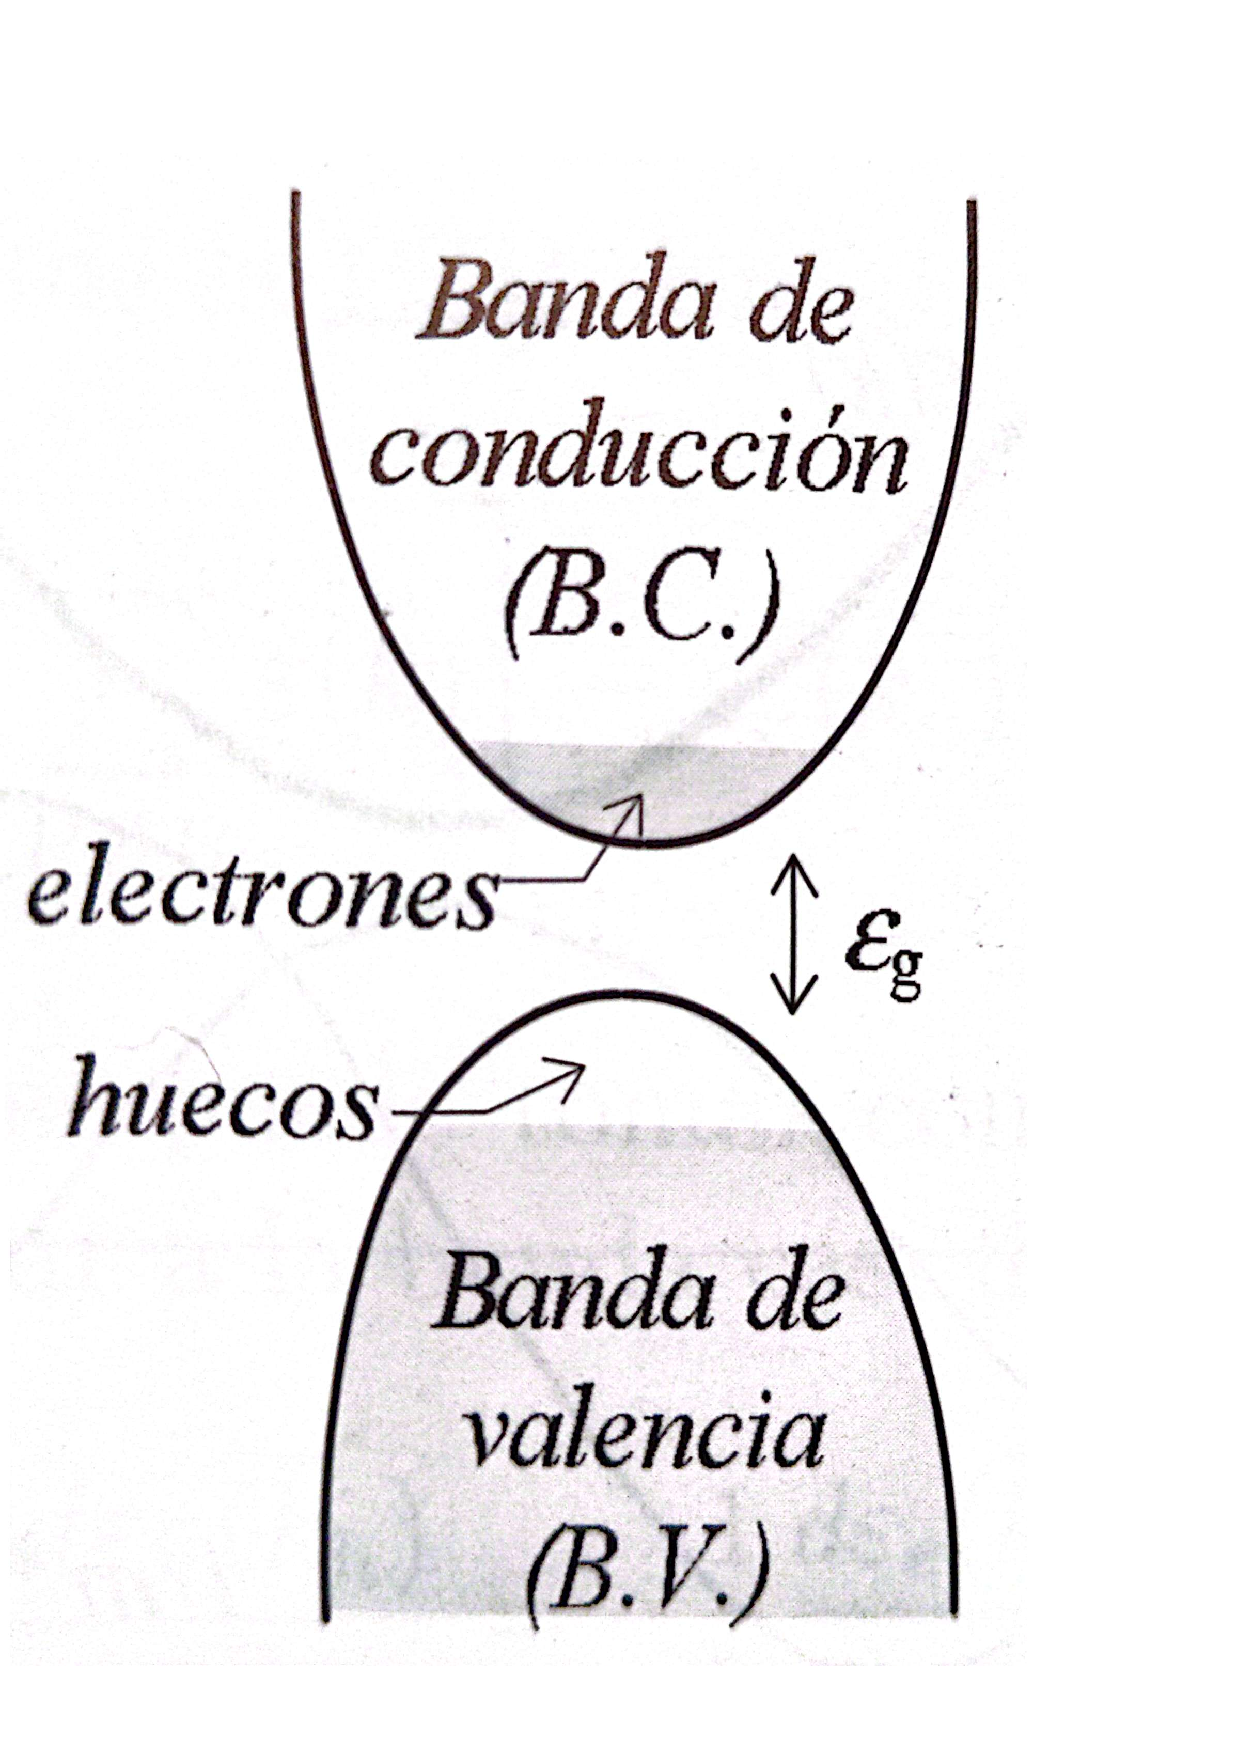
\includegraphics[scale=0.3]{Cuerpo/Ch_08/Fotos libro 1.pdf}
	\caption{Representación de los estados ocupados por electrones (en el fondo de la banda de conducción) y por huecos (en el techo de la banda de valencia) en un semiconductor.}
	\label{Fig:08-01}
\end{figure}


El concepto de masa cristalina se simplifica cuando se trata con electrones y huecos en los extremos de las bandas (figura \ref{Fig:08-01}), como es el caso de los semiconductores (capítulo \ref{Ch:09}). Si $\kn_0$ es el vector de onda asociado al extremo de una banda, podemos aproximar la energía en torno a $\kn_0$ según:

\begin{equation}
	\varepsilon(\kn) = \varepsilon(\kn_0) + \sum_{i,j} (k_i - k_{0i}) \frac{1}{2} \left. \parciales{^2 \varepsilon}{ k_i \partial k_j} \right|_{\kn=\kn_0} (k_j - k_{0j}) \label{Ec:08-02-04}
\end{equation} 
Por tanto la masa tensorial para un electrón que se mueve en las proximidades de $\kn_0$ será:

\begin{equation}
	\parentesis{\Mcal^{-1}}_{ij} = \frac{1}{\hbar^2} \left. \parciales{^2 \varepsilon}{ k_i \partial k_j} \right|_{\kn=\kn_0} = \cte
\end{equation}
y se habla entonces de \textit{masa efectiva}, denotada generalmente por $m^*$. En consecuencia, para semiconductores, para pasar de electrones libres a electrones de Bloch basta hacer la correspondencia $m\rightarrow m^*$, anisotropía aparte. Una simplificación adicional viene del carácter simétrico del tensor $m^*$ pues cabe tomar el sistema coordenado de modo que

\begin{equation}
	(m^*)^{-1} = \begin{pmatrix}
		1/m_1^* & 0 & 0 \\
		0 & 1/m_2^* & 0 \\
		0 & 0 & 1/m_3^* 
	\end{pmatrix} \ \Rightarrow (m^*) = \begin{pmatrix}
		m_1^* & 0 & 0 \\
		0 & m_2^* & 0 \\
		0 & 0 & m_3^* 
	\end{pmatrix} 
\end{equation}
y toda la dinámica del electrón en el externo de la banda viene controlada por tres masas efectivas $m_1^*,m_2^*,m_3^*$. La energía en (\ref{Ec:08-02-04}) se expresa entocnes por

\begin{equation}
	\varepsilon (\kn) = \varepsilon (\kn_0) + \frac{\hbar^2 (k_1-k_{01})^2}{2m_1^*} + \frac{\hbar^2 (k_2-k_{02})^2}{2m_2^*} + \frac{\hbar^2 (k_3-k_{03})^2}{2m_3^*}
\end{equation}
y entonces se ve que las superficies de energía $\varepsilon=\cte$ son elipsoides de semiejes:

\begin{equation}
	\frac{\sqrt{2m_1^* [\varepsilon-\varepsilon(\kn_0)]}}{\hbar} \quad 
	\frac{\sqrt{2m_2^* [\varepsilon-\varepsilon(\kn_0)]}}{\hbar} \quad
	\frac{\sqrt{2m_3^* [\varepsilon-\varepsilon(\kn_0)]}}{\hbar}
\end{equation}

\section{Movimiento en campos electricos. Concepto de hueco.}

Un importante resultante es que la densidad de corriente eléctrica de una banda llena es nula en presencias de campos externos. Por definición 

\begin{equation*}
	\jn \equiv - e \sum_i \vn_i= -e \hbar^{-1} \sum_i \parciales{\varepsilon}{\kn}
\end{equation*}
donde la suma es toda la PZB por la condición de banda llena. Como $\varepsilon(\kn)=\varepsilon(-\kn)$, se tiene que $\partial \varepsilon / \partial \kn |_\kn = - \partial \varepsilon / \partial \kn |_{-\kn}$, y los términos del anterior sumatorio se anulan por parejas ($\kn,-\kn$) ya que la PZB tiene simetría de inversión. El resultado anterior implica que hay tantos electrones que se mueven en la dirección $-\En$, como es de esperar para una carga negativa, como en la dirección $+\En$, como correspondería a una carga positiva. Para comprender este comportamiento consideremos la evolución de un solo electrón bajo efecto de un campo eléctrico $\En$ uniforme. La integración de (\ref{Ec:08-01-04}) es inmediata y da 

\begin{equation}
	\kn (t) = \kn(0) - \frac{e}{\hbar} \En t
\end{equation}
Si hacemos un esquema unidimensional, como se ilustra en la figura \ref{Fig:08-02}, deducimos que el movimiento del electrón en $\kn$ es periódico (y también lo es en el espacio real, pues si $\varepsilon$ es periódico también lo es $\vn \propto \partial \varepsilon / \partial \kn$ y por tanto la posición). Conforme el electrón se acerca a la frontera de zona presenta un comportamiento anómalo asociado a su masa efectiva \textit{negativa} en esa región. En realidad este comportamiento no es observable debido a las colisiones,  que mantienen al electrón alrededor del fondo de la banda, donde el comportamiento es ``normal''. Naturalmente, el comportamiento del electrón a la combinación Fuerzas externas+Potencial cristalino es completamente normal.

\begin{figure}[h!] \centering
	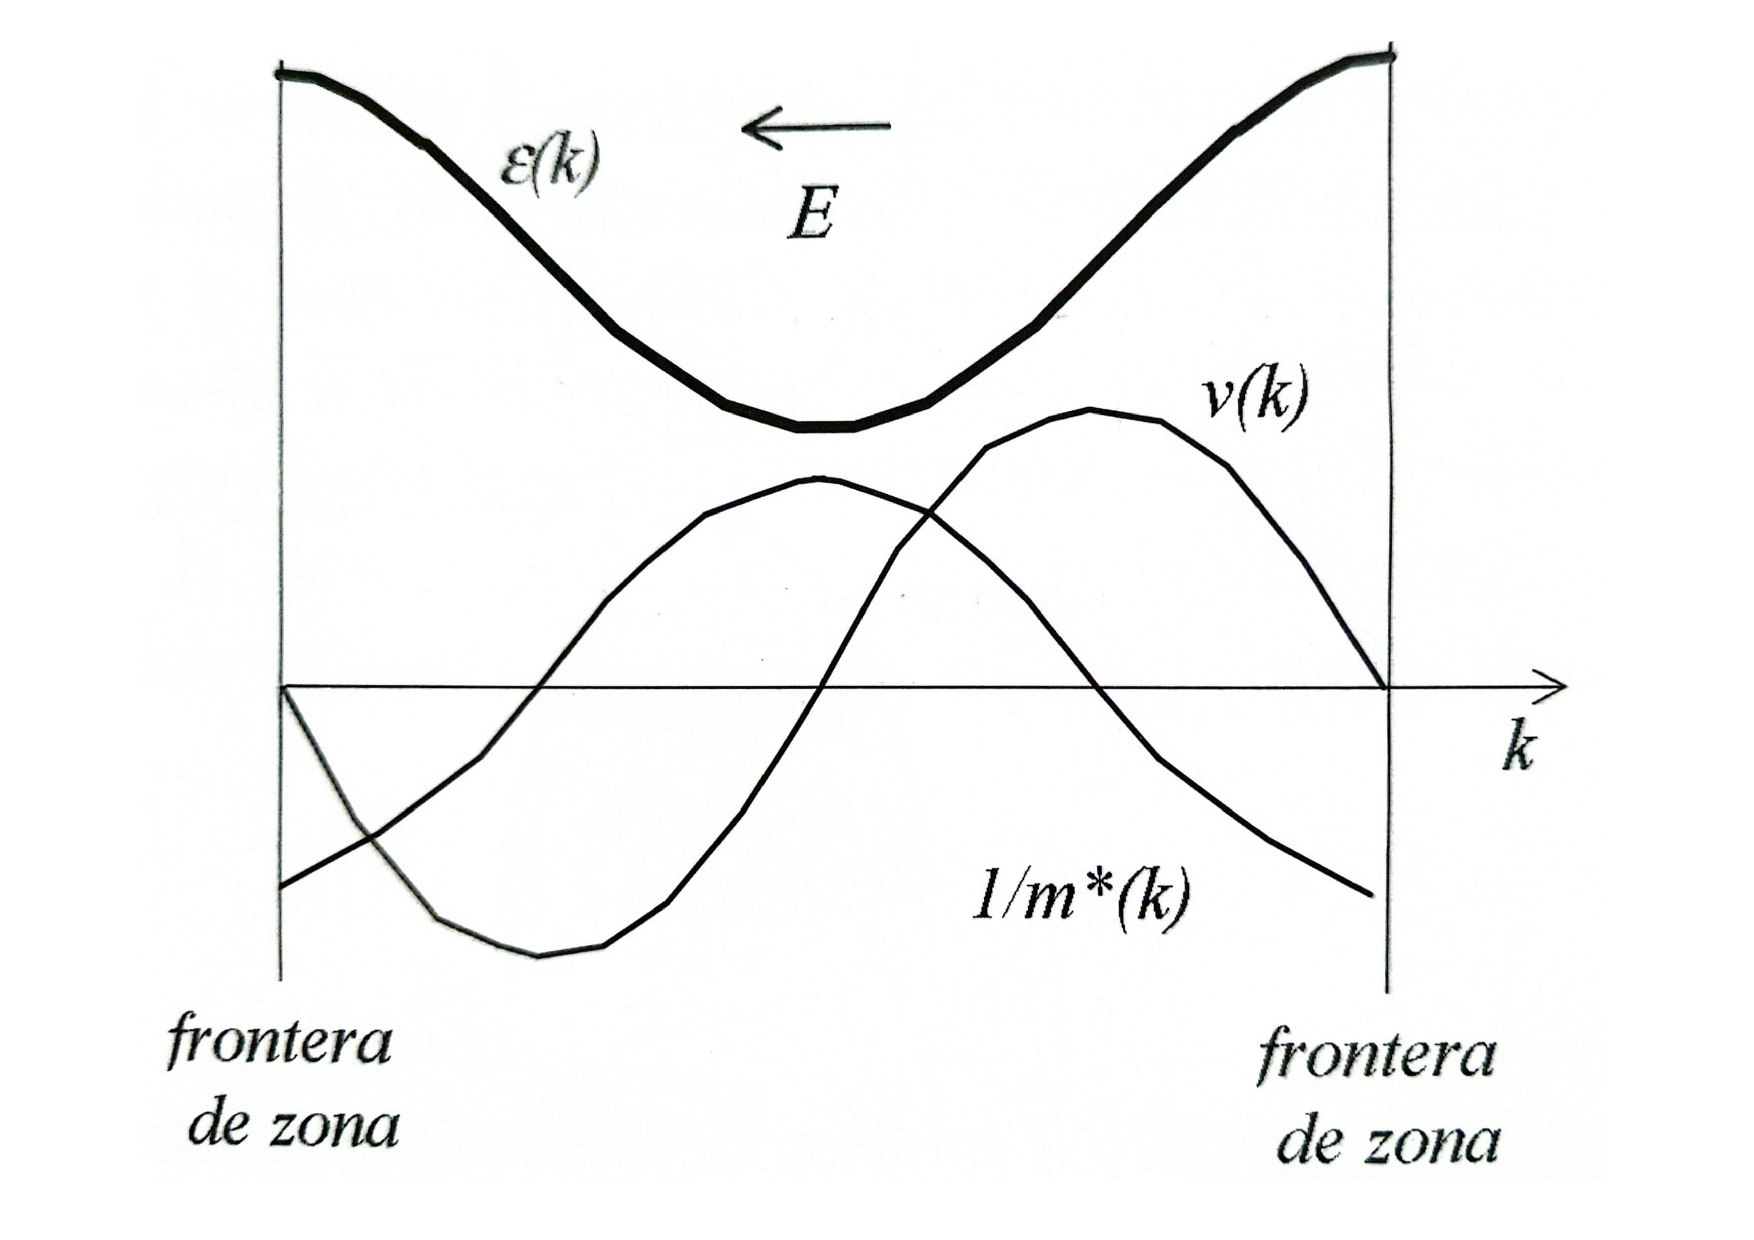
\includegraphics[scale=0.35]{Cuerpo/Ch_08/Fotos libro 2.pdf}
	\caption{Energía, masa efectiva y velocidad de un electrón según su posición en la PZB. Nótense los estados ``anómalos'' (con masa efectiva negativa) cerca de las fronteras de zona.}
	\label{Fig:08-02}
\end{figure}

A diferencia del ejemplo anterior, los estados ``anómalos'' son obsevables en la situación de una banda casi llena. Para simplificar consideremos una banda con un solo estado electrónico vacante respeto con el vector de onda $\kn_e$, en cuyo casi diremos que existe un \textit{hueco}. Veamos la respuesta global de la banda frente a campos eléctricos. Denotaremos con subíndice $h$ las magnitudes de banda, y con $e$ las del estado electrónico ausente. Respecto al vector de onda que asociar a la banda:

\begin{equation}
	\kn_h \equiv \parentesis{\sum_{PZB} \kn} - \kn_e = - \kn_e
\end{equation}
pues $\parentesis{\sum_{PZB} \kn} =0$ por simetría de la PZB. En lo que respecta a la energía 

\begin{equation}
	\varepsilon_h (\kn_h) \equiv \ccorchetes{\sum_{PZB} \varepsilon(\kn) } - \varepsilon_e (\kn_e) = - \varepsilon_e (\kn_e)
\end{equation}
pues la constante $\sum_{PZB} \varepsilon(\kn)$ se puede tomar como cero. A partir de $\kn_h$ y $\varepsilon_h$ la velocidad $\vn_h$ que se debe asociar a la banda casi llena es 
 
\begin{equation}
	\vn_h (\kn_h) \equiv \frac{1}{\hbar} \derivadas{\varepsilon_h (\kn_h)}{\kn_h} = - \frac{1}{\hbar} \derivadas{\varepsilon_e (\kn_e)}{(-\kn_e)} = \vn_e (\kn_e)
\end{equation}
En cuanto masa efectiva

\begin{equation}
	m_h^{-1} \equiv \frac{1}{\hbar^2} \derivadas{^2\varepsilon_h (\kn_h)}{\kn_h^2} = - \frac{1}{\hbar^2} \derivadas{^2\varepsilon_e (\kn_e)}{(-\kn_e)^2} = - m_e^{-1}(\kn_e)
\end{equation}
de donde se deduce que la masa efectiva del hueco es positiva, por tratase de un estado electrónica cerca del techo de la banda, donde $1/m_e \propto \D^2 \varepsilon_e / \D \kn_e <0$. Si aplicamos ahora la ecuación dinámica (\ref{Ec:08-01-04}) al electrón ausente $\hbar \D \kn_e / \D t = - e (\En + \vn_e \times \Bn)$, al sustituir $\kn_e$ por $-\kn_h$ y $\vn_e$ por $\vn_h$ obtenemos:

\begin{equation}
	\hbar \derivadas{\kn_h}{t} = - e (\En + \vn_h \times \Bn)
\end{equation}
de donde se ve que un hueco se comporta como una partícula de carga eléctrica \textit{positiva} con masa positiva. Finalmente, la conductividad eléctrica de una banda parcialmente llena viene dada por

\begin{equation}
	\sigma = \frac{e^2 \tau}{V} \sum_{\kn} \Mcal^{-1} (\kn)
\end{equation}
donde la suma se extiende a todos los estados ocupadas en la banda. Esta expresión es una generalización vista en el Capítulo \ref{Ch:07} para $e^-$ libres. En efecto, para electrones libres $\Mcal^{-1} (\kn) = m^{-1}$, con lo que $\sigma = e^2 \tau N / V m = ne^2 \tau / m$.

\section{Movimiento en campos magnéticos.}

Bajo un campo magnético la fuerza que actúa sobre los portadores $q\vn \times \Bn$, por ser perpendicular a $\vn$, conserva la energía electrónica:

\begin{equation}
	\derivadas{\varepsilon}{t} = \Fn \cdot \vn = 0 \ \Rightarrow \ \varepsilon(\kn) = \cte
\end{equation}
Otra ley de conservación se deduce de la ecuación dinámica 

\begin{equation*}
	\hbar \derivadas{\kn}{t} = - e \vn \times \Bn
\end{equation*}
En efecto, descomponiendo $\kn$ en sus componentes paralela y perpendicular a $\Bn$ ($\kn = \kn_\perp + \kn_\parallel $) se tendrá $(\vn \times \Bn)_\parallel =0$, de donde $\kn_\parallel=\cte$. Por tanto, en un campo magnético los electrones se mueven a lo largo de las curvas de intersección de las superficies de energía constante con planos perpendiculares al campo magnético aplicado (ver Fig. \ref{Fig:08-03})

\begin{figure}[h!] \centering
	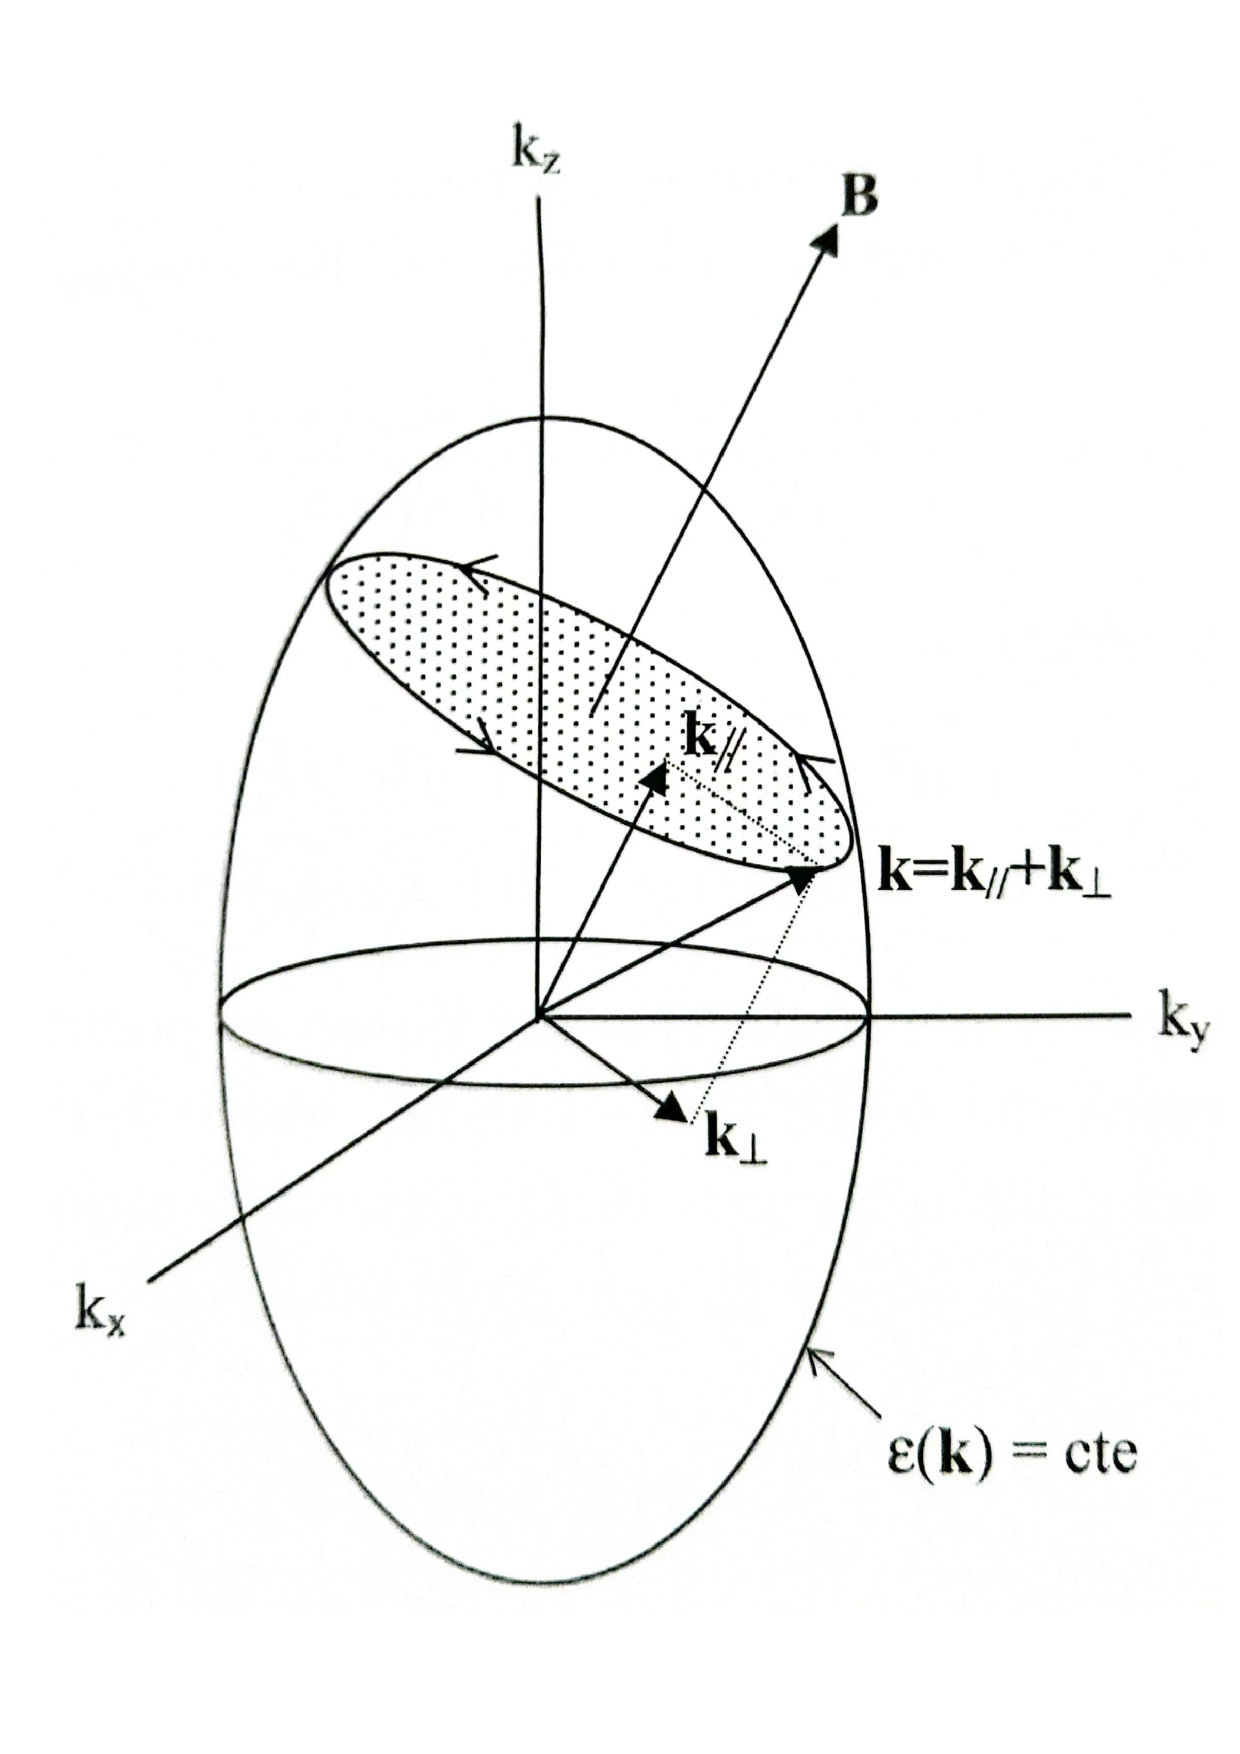
\includegraphics[scale=0.35]{Cuerpo/Ch_08/Fotos libro 3.pdf}
	\caption{Movimiento de un electrón en el espacio de fases bajo influencia de un campo magnético.}
	\label{Fig:08-03}
\end{figure}

Veamos ahora cómo son las órbitas en el espacio real. La proyección de $\hbar \D \kn / \D t = - e \vn \times \Bn$ en la dirección perpendicular a $\Bn$ da:

\begin{equation}
	\hnn \times \hbar \derivadas{\kn_\perp}{t} = - e \hnn \times (\vn_\perp \times \Bn) = - e B \vn_\perp
\end{equation}
Como $\D \rn_\perp / \D t = \vn_\perp$ , la ecuación anterior se integra fácilmente para dar 

\begin{equation}
	\rn_\perp (t) = \rn_\perp (0) - \hnn \times \frac{\hbar}{eB} \ccorchetes{ \kn_\perp (t) - \kn_\perp (0)}
\end{equation}
cuya interpretación es que la proyección perpendicular a $\Bn$ de la órbita en el espacio real no es sino la órbita en el espacio $\kn$ girada $\pi/2$ alrededor de la dirección de $\Bn$ y escalada en el factor $-\hbar / eB$. Por su parte, la velocidad paralela al campo vendrá dada por $\vn_\parallel=\hbar^{-1} \D \varepsilon/\D \kn_\parallel$, que no tiene por qué ser constante. 

Hay, como ilustra la figura \ref{Fig:08-04} en un ejemplo 2D, órbitas \textit{tipo electrón} y \textit{tipo hueco} que difieren por el sentido de recorrido, pues la velocidad es opuesta al serlo el gradiente de energía (aunque en ambos casos son electrones los que describen las órbitas). Como regla general, las órbitas que encierran estados desocupados son tipo huevo, y las que encierran estados ocupados son de tipo electrón.

\begin{figure}[h!] \centering
	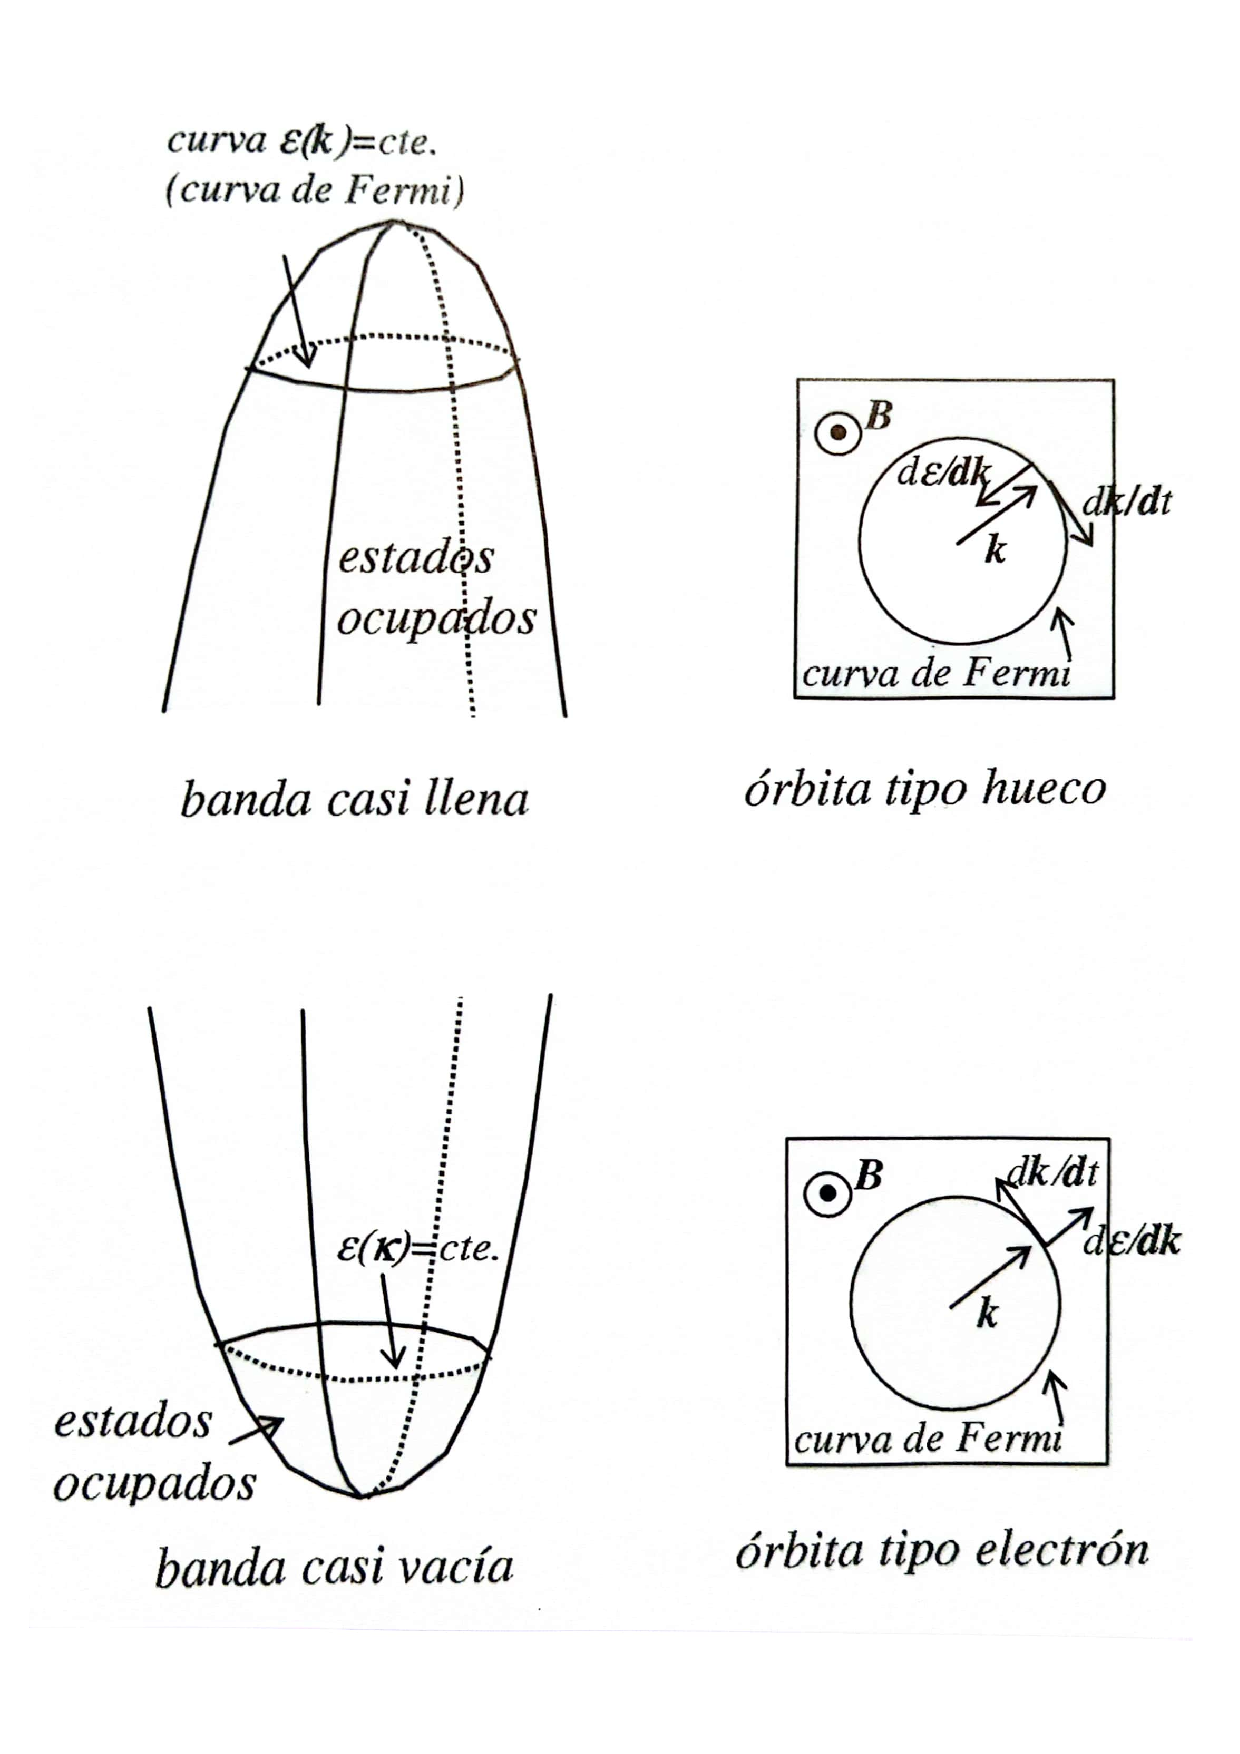
\includegraphics[scale=0.5]{Cuerpo/Ch_08/Fotos libro 4.pdf}
	\caption{Órbitas en el espacio de fases de electrones y de huecos bajo la influencia de un campo mangético.}
	\label{Fig:08-04}
\end{figure}

\subsection{Resonancias ciclotrón: determinación experimental de masas efectivas.}

Las órbitas (cerradas) electrónicas naturalmente periódica con período (pag. 231 \textit{Ashcroft and Mermin} \cite{Mermin_Solid_State})

\begin{equation}
	T(\varepsilon,k_\parallel) = \frac{\hbar^2}{eB} \parciales{}{\varepsilon}\parentesis{A(\varepsilon,k_\parallel)}
\end{equation}
siendo $A(\varepsilon,k_\parallel)$ el área encerrada por la órbita (en el espacio de fases). Este período es una propiedad de toda la órbita, no de un estado electrónico particular. La frecuencia $\omega_c (\varepsilon,k_\parallel)=2\pi/T(\varepsilon,k_\parallel)$ se denomina \textit{frecuencia ciclotrón}, y es una generalización de la frecuencia ciclotrón del electrón libre ($\omega_c = e B/m$). Por comparación con esta última expresión, se introduce

\begin{equation}
	m^* (\varepsilon,k_\parallel) = \frac{eB}{\omega_c (\varepsilon,k_\parallel)} = \frac{\hbar^2}{2\pi} \parentesis{A(\varepsilon,k_\parallel)}{\varepsilon}
\end{equation}
que se conoce como \textit{masa efectiva ciclotrónica}, cuyo valor depende de la masa efectiva (vista anteriormente, y con la que no debe de confundirse, pues la masa efectiva ciclotrónica es una propiedad de toda la órbita y no de un estado individual).

Para estados cerca de los extremos de bandas, de interés en los semiconductores, es fácil demostrar que $\omega_c$ puede expresarse por

\begin{equation}
	\omega_c = e \parentesis{\frac{B_1^2 m_1^* + B_2^2 m_2^* + B_3^2 m_3^*}{m_1^* m_2^* m_3^*}}^{1/2} \label{Ec:03-04-06}
\end{equation}
donde las $B_i$ son las componentes de $\Bn$ a lo largo de los ejes principales del elipsoide $\varepsilon(\kn) = \cte$, y $m_1^*,m_2^*,m_3^*$ las correspondientes componentes del tensor de masa efectiva. La ecuación (\ref{Ec:08-04-06}) permite acceder experimentalmente a las masas efectivas de los electrones y huecos en semiconductores. La determinación experimental de $\omega_c$  se realiza por resonancia con un campo electromagnético de frecuencia adecuada. En concreto se detectan los máximos de absorción de una onda electromagnética polarizada circularmente aplicada en la dirección de un campo magnético externo estático y homogéneo (el único requisito es que las colisiones no impidan observar el efecto, esto es, que se cumpla $\omega_c \tau > 1$ lo que exige trabajar a bajas temperaturas).

\subsection{Magnetorresistividad y efecto Hall}

En campos magnéticos débiles ($\omega_c \tau \ll 1$) de forma que el electrón sólo recorre una pequeña parte de su órbita cerrada entre colisiones, la resistencia crece proporcionalmente al cuadrado del campo magnético. Esto es de esperar ya que, en primer lugar, la magnetorresistividad $\rho(\Bn)-\rho(0)$ debe ser siempre positiva pues el campo magnético siempre dificultará en alguna medida el movimiento longitudinal de los portadores. Esto descarta la dependencia lineal $\Bn$, que implica un cambio de signo en la magnetorresistividad al cambiar $\Bn$ de signo, de modo que $\rho(\Bn)$ debe depender cuadráticamente de $\Bn$. 

Para ver el comportamiento de la magnetorresistividad como del efecto Hall debe estudiarse el transporte de corriente bajo campo eléctrico y magnético aplicados simultáneamente. En presencia de campos $\En\perp\Bn$, la densidad de corriente se puede escribir como 

\begin{equation}
	\jn = \sigma_E \En + \sigma_B (\Bn \times \En) \label{Ec:03-04-07}
\end{equation}
donde tanto $\sigma_E$ como $\sigma_B$ son escalares que dependen de la concentración de portadores, de su masa efectiva, de su tiempo de relajación y del campo magnético. Considerando $\Bn=(0,0,B)$ y $\En=(E_x,E_y,0)$ la ecuación (\ref{Ec:03-04-07}) puede escribirse como

\begin{equation}
	\jn = \sigma (B) \En = \begin{pmatrix}
	\sigma_E & - B\sigma_B & 0 \\ 
	B \sigma_B & \sigma_E & 0 \\
	0 & 0 & 1 
	\end{pmatrix} \En
\end{equation}
en régimen estacionario ($j_y = 0$) se obtiene, respectivamente, para la Magnetorresistividad y el coeficiente Hall

\begin{equation}
	\rho = \frac{E_z}{j_x} = \frac{\sigma_E}{\sigma_E^2+\sigma_B^2 B^2} \tquad R = \frac{E_y}{j_xB} =  \frac{-\sigma_B}{\sigma_E^2 + \sigma_B^2 B^2}
\end{equation}
Para la aproximación más simple, es decir, electrones \textit{cuasilibres}:

\begin{equation*}
	\sigma_E = \frac{ne^2 \tau/m^*}{1+(\omega_c\tau)^2} \tquad \omega_B = \frac{e\tau}{m^*} \sigma_E  \tquad (\omega_c = eB/m^*)
\end{equation*}
con lo cual 

\begin{equation}
	\rho = \frac{m^*}{ne^2\tau} = \rho(0) \quad R=-\frac{1}{ne}
\end{equation}
En el caso de existir varios portadores, incluso la aproximación más simple, es decir, $\rho(\Bn)=\rho_i(0)$ para cada uno de los portadores $i$, sí se obtendría una magnetorresistividad global.

Suponiendo que las superficies equienergéticas (en particular la de Fermi) son esferas \textit{ligeramente} deformadas, se puede aproximar

\begin{equation}
	\sigma (B) \approx \frac{ne^2 \tau}{m^*} \begin{pmatrix}
	1-5 (\omega_c \tau)^2 & -2\omega_c \tau & 0 \\
	2 \omega_c \tau & 1-5(\omega_c \tau)^2 & 0 \\
	0 & 0 & 1
	\end{pmatrix}
\end{equation}
con lo cual (en régimen estacionario)

\begin{equation}
	\rho(B) \approx \rho(0) \ccorchetes{1+(\omega_c \tau)^2} \Rightarrow \frac{\rho(B)-\rho(0)}{\rho(0)} \propto B^2
\end{equation}
Para el coeficiente Hall se obtendría 

\begin{equation}
	R \approx - \frac{1}{ne} \ccorchetes{1+3(\omega_c \tau)^2}
\end{equation}
Obsérvese que para $B\rightarrow 0$ se reencuentran los resultados del electrón libre. En campos magnéticos intensos ($\omega_c \tau \gg 1$) la magnetorresistividad presenta una gran variedad de comportamientos dependiendo de la topología de la superficie de Fermi: puede saturar para todas las direcciones de $\Bn$, solo para algunas puede crecer indefinidamente con el campo implica la existencia de órbitas \textit{abiertas}.

En cuanto al coeficiente Hall, a campos altos resulta válida la expresión de electrones libres, sólo que la concentración de electrones $n_e$ se sustituyen por la concentración neta de portadores ($n_e-n_h$) siendo $n_h$ la concentración de huecos, es decir

\begin{equation}
	R_H = - \frac{1}{e(n_e-n_h)}
\end{equation}
en el caso de que $n_e=n_eh$ (los llamados \textit{metales compensados}) la expresión anterior no es válida-